\documentclass[a4paper]{article}
\usepackage{ctex}
\usepackage{enumitem}
\usepackage{fancyhdr}
\usepackage{amsmath}
\usepackage{parskip}
\usepackage{float}
\usepackage{listings}
\usepackage{hyperref}
\usepackage{xcolor}

\setlength{\parskip}{6pt}

\pagestyle{headings}

\begin{document}
\title{计数器的设计}
\author{梁业升 2019010547(计03)}

\maketitle

% GitHub styles
\definecolor{keyword}{HTML}{CF222E}
\definecolor{comment}{HTML}{6E7781}
\definecolor{string}{HTML}{0A3069}

\lstset{
    commentstyle=\color{comment},
    keywordstyle=\color{keyword},
    stringstyle=\color{string},
    basicstyle=\ttfamily\small,
    breakatwhitespace=false,
    breaklines=true,
    captionpos=b,
    keepspaces=true,
    showspaces=false,
    showstringspaces=false,
    showtabs=false,
}


\section{实现}
\subsection{触发器}

\begin{lstlisting}[language=vhdl]
library ieee;
use ieee.std_logic_1164.all;
use ieee.std_logic_arith.all;
use ieee.std_logic_unsigned.all;

entity ff is
    port(
        clk, rst, pause: in std_logic;
        n1, n0: buffer std_logic_vector(3 downto 0) -- 十位和个位
    );
end ff;

architecture arch of ff is
begin
    process(clk, rst)
    begin
        if (rst = '1') then
            n0 <= "0000";
            n1 <= "0000";
        elsif (clk'event and clk = '1' and pause = '0') then
            if (n0 = "1001") then -- X9
                n0 <= "0000"; -- 个位置零
                if (n1 = "0101") then -- 59
                    n1 <= "0000"; -- 十位置零
                else
                    n1 <= n1 + 1;
                end if;
            else
                n0 <= n0 + 1;
            end if;
        end if;
    end process;
end arch;
\end{lstlisting}

因为需要以十进制输出,所以需要分别储存两位的二进制表示,并在个位达到 9 或总数达到 59 时置零。另外,对 \texttt{pause} 信号作判断,
当 \texttt{pause} 为 1 时,不进行计数。

\subsection{七位数码管显示}

\begin{lstlisting}[language=vhdl]
library IEEE;
use IEEE.STD_LOGIC_1164.ALL;
use IEEE.STD_LOGIC_ARITH.ALL;
use IEEE.STD_LOGIC_UNSIGNED.ALL;

entity digital_7 is
    port(
        number: in std_logic_vector(3 downto 0);
        display: out std_logic_vector(0 to 6)
    );
end digital_7;

architecture bhv of digital_7 is
begin
    process(number)
    begin
        case number is
            when "0000" => display <= "1111110";
            when "0001" => display <= "0110000";
            when "0010" => display <= "1101101";
            when "0011" => display <= "1111001";
            when "0100" => display <= "0110011";
            when "0101" => display <= "1011011";
            when "0110" => display <= "1011111";
            when "0111" => display <= "1110000";
            when "1000" => display <= "1111111";
            when "1001" => display <= "1110011";
            when "1010" => display <= "1110111";
            when "1011" => display <= "0011111";
            when "1100" => display <= "1001110";
            when "1101" => display <= "0111101";
            when "1110" => display <= "1001111";
            when "1111" => display <= "1000111";
            when others => display <= "0000000";
        end case;
    end process;

end bhv;
\end{lstlisting}

此元件直接使用“点亮数字人生”中的代码。

\subsection{计数器}

\begin{lstlisting}[language=vhdl]
library ieee;
use ieee.std_logic_1164.all;
use ieee.std_logic_arith.all;
use ieee.std_logic_unsigned.all;

entity counter is
    port(
        clk, rst, pause: in std_logic;
        n0, n1: buffer std_logic_vector(3 downto 0);
        hi, lo: out std_logic_vector(0 to 6) -- 十位和个位
    );
end counter;

architecture arch of counter is
    component ff
        port(
            clk, rst, pause: in std_logic;
            n1, n0: buffer std_logic_vector(3 downto 0)
        );
    end component;
    
    component digital_7
        port(
            number: in std_logic_vector(3 downto 0);
            display: out std_logic_vector(0 to 6)
        );
    end component;
    
    signal qs: std_logic_vector(0 to 5) := "000000";
    signal nqs: std_logic_vector(0 to 5) := "111111";
    signal cnt: integer := 0;
    signal real_clk: std_logic := '0'; -- 触发器使用的时钟信号
begin
    ff0: ff port map(clk=>real_clk, rst=>rst, pause=>pause, n0=>n0, n1=>n1);
    
    display0: digital_7 port map(number=>n0, display=>lo); -- 个位
    display1: digital_7 port map(number=>n1, display=>hi); -- 十位
    
    process(clk)
    begin
        if (clk'event and clk = '1') then
            if (cnt < 500000) then
                cnt <= cnt + 1;
            else
                cnt <= 0;
                real_clk <= (not real_clk); -- 反转时钟信号
            end if;
        end if;
    end process;
    
end arch;
\end{lstlisting}

为了做到使用 1MHz 时钟进行自动计数,我们在计数器元件中记录时钟上升沿次数 \texttt{cnt},当 \texttt{cnt} 等于 1M/2 = 500000 时
改变触发器所使用的时钟信号 \texttt{real\_clk},这样就实现了 1 秒计 1 次数。


\section{实验结果}

\subsection{仿真结果}

\begin{figure}[H]
    \centering
    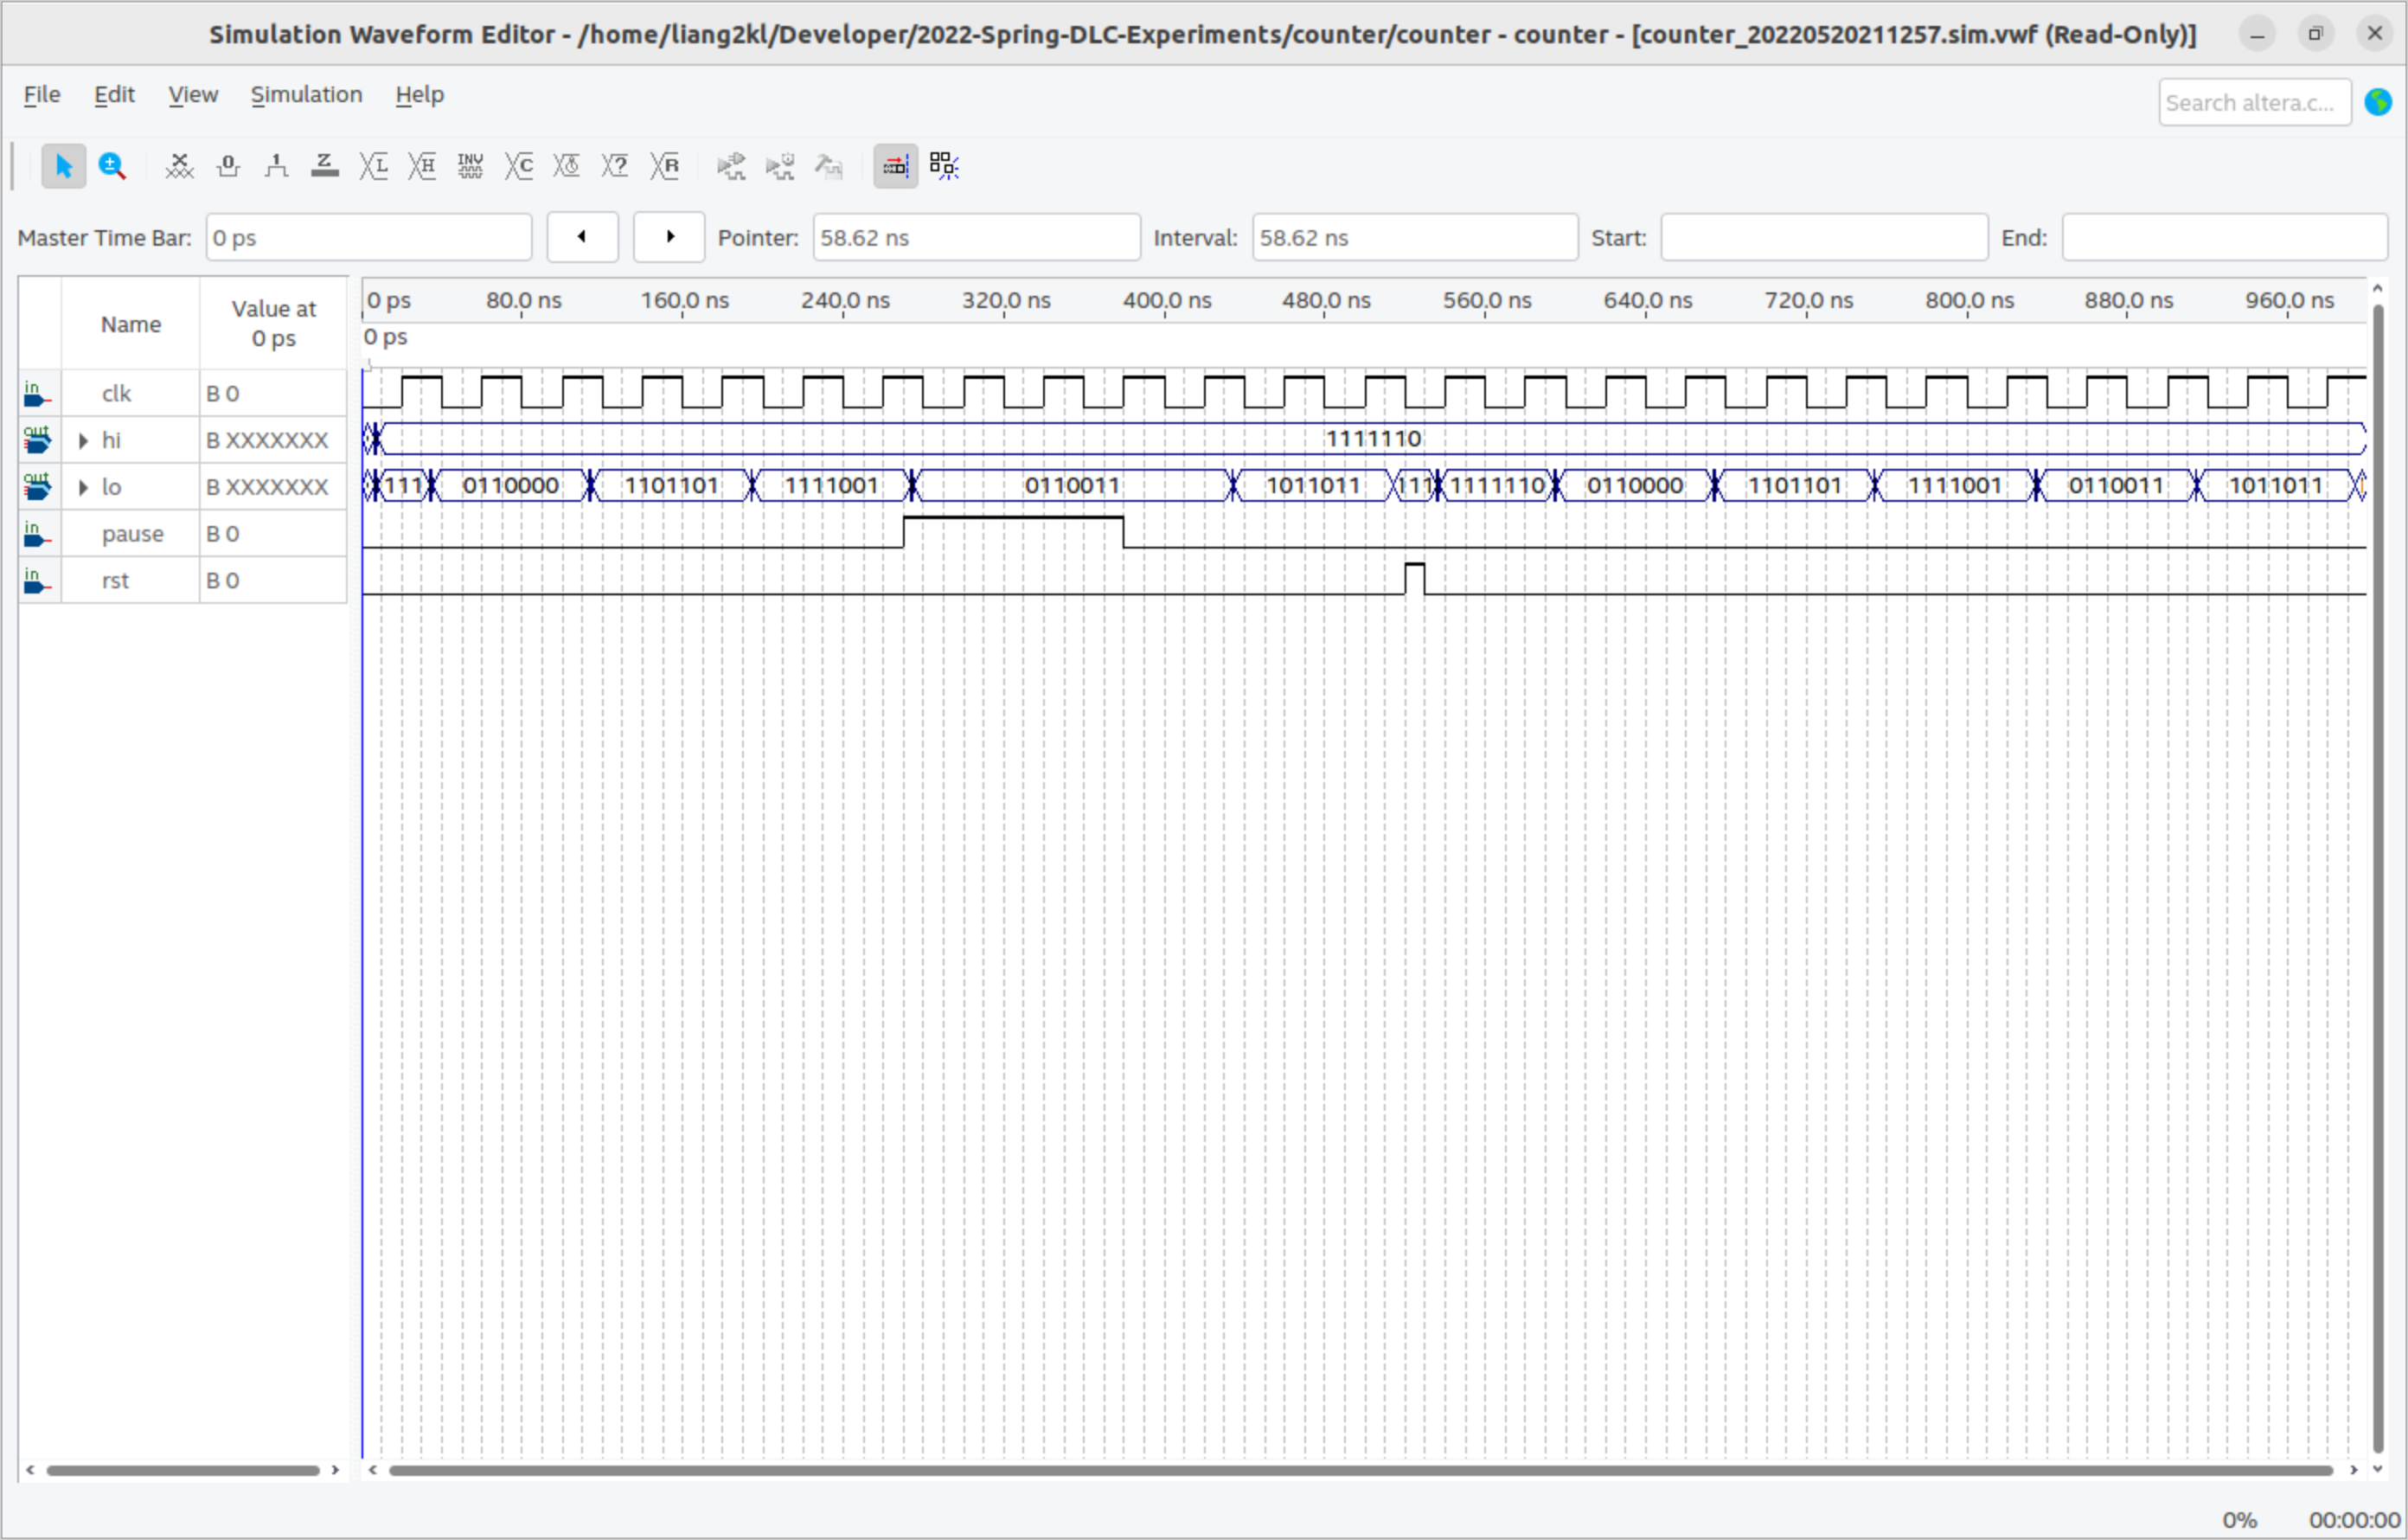
\includegraphics[width=1\textwidth]{./assets/simulation.png}
\end{figure}

可以看到,计数、复位和暂停功能均正常。

\subsection{实际操作结果}

计数器能够自动计数,并能正确处理复位和暂停信号。

\section{实验总结}

由于有了第一次实验的基础,本次实验代码编写进展比较顺利,没有遇到较大的问题。使用了元件例化的方法,体验了结构化设计
的好处。

\end{document}
